
\section{Preprocessing and Data Visualization}
\label{sec:DatasetAndPreprocessing}

\subsection{Dataset Description}

This project utilizes the "Twitter Entity Sentiment Analysis" dataset from Kaggle \cite{twitter_dataset}. This dataset provides a collection of tweets, each associated with a specific entity and annotated with a sentiment label, serving as a robust foundation for training and evaluating sentiment analysis models.

The raw data for training and validation was initially loaded with columns subsequently renamed for clarity to: `tweetID`, `entity`, `sentiment`, and `tweet\_content`.

The initial preparation steps involved:
\begin{enumerate}
    \item \textbf{Standardizing Sentiment Labels}: Sentiment labels in both training and validation sets were converted to lowercase (e.g., 'Positive' to 'positive').
    \item \textbf{Filtering Sentiments}: Only tweets with 'positive', 'negative', or 'neutral' sentiments were retained, excluding any irrelevant or ambiguous sentiment labels.
    \item \textbf{Handling Missing Values}: Rows with any missing values (`NaN`) were removed.
    \item \textbf{Removing Duplicates}: Duplicate rows were removed  to ensure data integrity.
\end{enumerate}

After these initial cleaning steps, the dataset consists of tweets where `tweetID` is a unique identifier for the tweet, `entity` refers to the specific named entity the tweet discusses, `sentiment` is the classified sentiment (positive, negative, or neutral), and `tweet\_content` contains the raw text of the tweet. This structured and cleaned dataset is then used for exploratory analysis and model training, with the goal of accurately classifying tweet sentiment across various entities.

\subsection{Exploratory Data Analysis (EDA)}
To understand the characteristics of the dataset, an exploratory data analysis was conducted.

\subsubsection{Distribution of Entities}

The distribution of entities Fig.\ref{fig:entity_distribution} within the dataset was examined. 

\begin{figure}[h!]
    \centering
    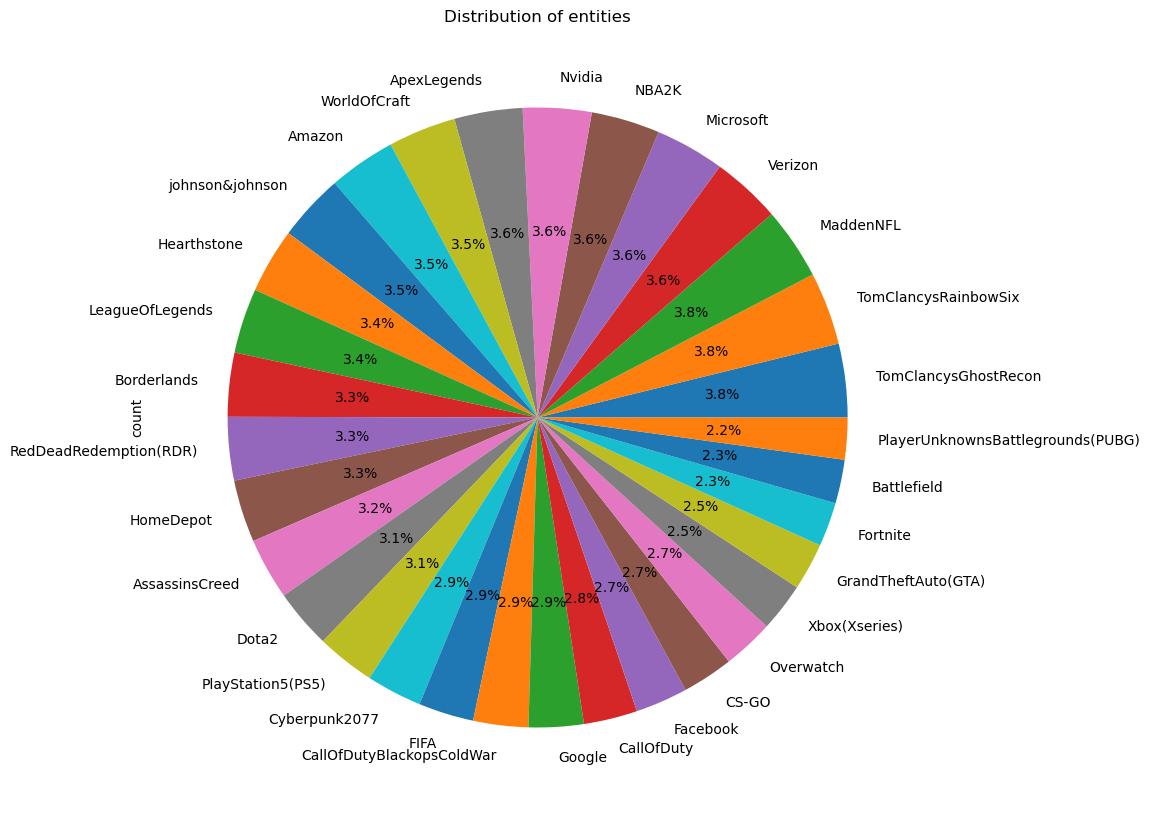
\includegraphics[width=1\linewidth]{images/entity_distribution.png}
    \caption{distribution of entities}
    \label{fig:entity_distribution}
\end{figure}

A pie chart visualizing the frequency of each entity revealed that the entities are relatively uniformly represented, with most entities comprising around 3\% of the dataset each. This near-uniform distribution is beneficial as it suggests that the dataset is not heavily skewed towards a small number of entities, allowing models to learn from a diverse range of subjects.



\subsubsection{Distribution of Sentiment Labels}

The overall distribution of sentiment labels (positive, negative, neutral) was analyzed Fig.\ref{fig:sentiment_distribution}. 

\begin{figure}[H]
    \centering
    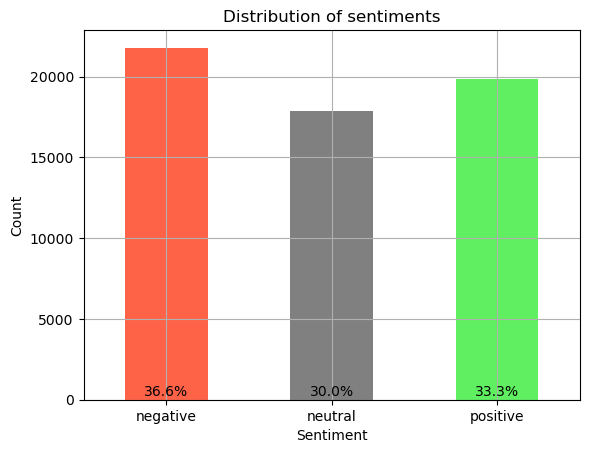
\includegraphics[width=1\linewidth]{images/sentiment_distribution.png}
    \caption{Sentiment Distribution}
    \label{fig:sentiment_distribution}
\end{figure}


A bar chart showed the following approximate distribution:

\begin{itemize}
    \item Negative: Around 36%
    \item Positive: Around 33%
    \item Neutral: Around 30%
\end{itemize}

These proportions indicate that the dataset is reasonably balanced across the three sentiment classes. This balance is crucial for training unbiased models, as it prevents the model from being skewed towards a majority class and helps ensure fair performance evaluation across all sentiments.


\subsubsection{Sentiment Distribution per Entity}

To delve deeper, the sentiment distribution for each individual entity was investigated, Fig.\ref{fig:sentiment_per_entity} 

\begin{figure}[h!]
    \centering
    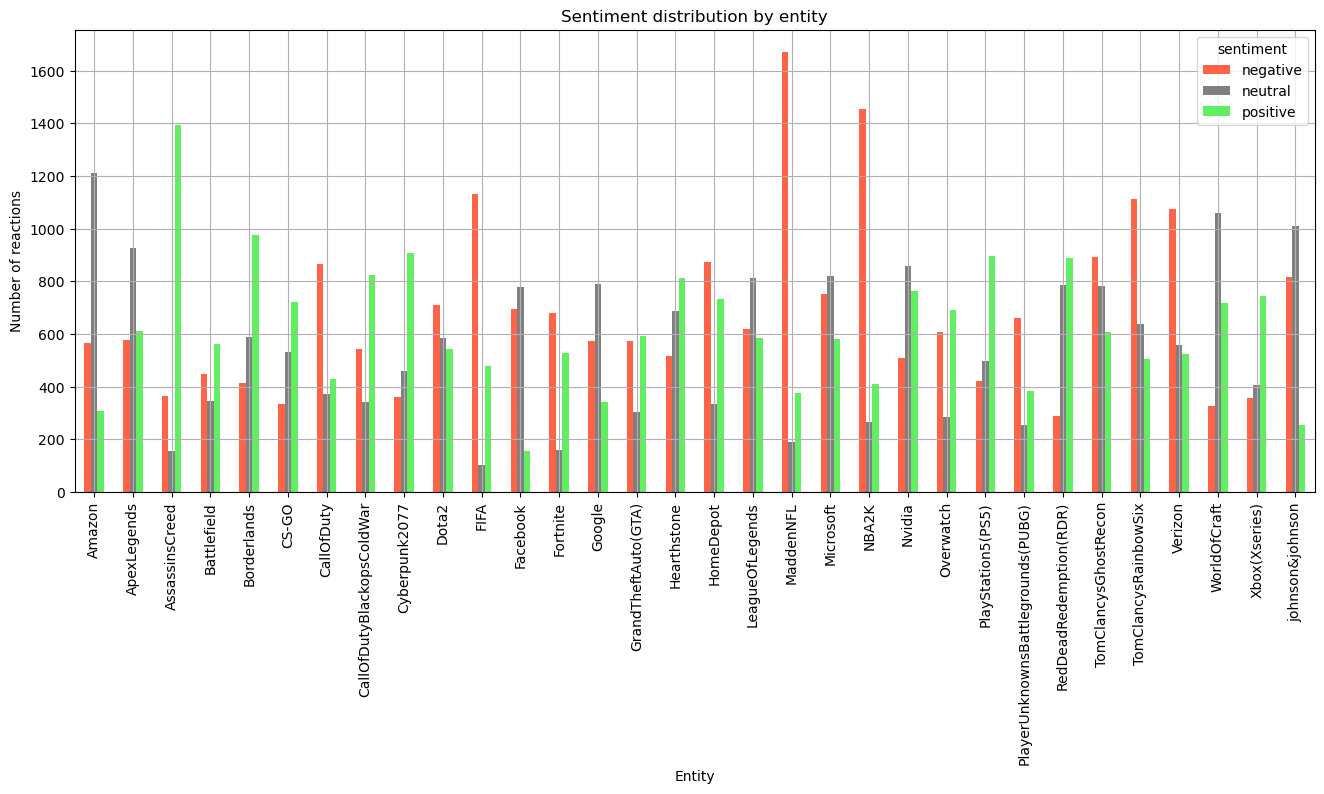
\includegraphics[width=1\linewidth]{images/sentiment_per_entity.png}
    \caption{Sentiment per Entity}
    \label{fig:sentiment_per_entity}
\end{figure}

A grouped bar chart illustrating the number of positive, negative, and neutral reactions for each entity provided valuable insights. For example, it was observed that:
\begin{itemize}
    \item The entity "Madden NFL" tended to have a higher proportion of negative reactions.
    \item "Assassin's Creed" showed a tendency towards more positive reactions.
    \item "Amazon" exhibited a significant number of neutral reactions.
    \item Entities like "Tom Clancy's Ghost Recon" had a more mixed sentiment profile, with comparable numbers of positive, negative, and neutral reactions.
\end{itemize}

This analysis highlights that sentiment can be entity-dependent and showcases the nuanced nature of the dataset. Understanding these entity-specific sentiment patterns is important for interpreting model behavior and identifying potential areas where models might struggle or excel.

\subsection{Text Preprocessing}

Twitter text is inherently noisy, containing slang, abbreviations, URLs, user mentions, hashtags, emojis, and other elements that can hinder the performance of Natural Language Processing (NLP) models. Therefore, a comprehensive text preprocessing was applied to clean and normalize the `tweet\_content` before it was fed into the machine learning and deep learning models.

\begin{enumerate}
    \item Handling Missing Values and Type Conversion: Initially, any `NaN` (Not a Number) entries in the tweet content are converted to empty strings to prevent errors in subsequent processing. The text is then explicitly converted to a string data type.
    \item Removing Web Elements:
     \begin{itemize}
     \item \textbf{URLs}: All HTTP and HTTPS links (e.g., `http://example.com` or `www.example.com`) are removed as they typically do not contribute to the sentiment of the text itself.
     \item \textbf{Mentions}: Twitter mentions (e.g., `@username`) are stripped from the text to remove user-specific addressing.
     \item \textbf{Hashtags}: The '\#' symbol is removed from hashtags, but the textual content of the hashtag is retained (e.g., `\#topic` becomes `topic`), as the hashtag text can often carry sentiment or important keywords.
     \end{itemize}
    \item Character Cleaning and Normalization:
     \begin{itemize}
    \item  \textbf{Emojis and Non-Text Symbols}: Emojis and most other non-text symbols are removed. The process aims to eliminate characters that are not alphanumeric or standard whitespace, while attempting to preserve accented characters common in various languages (e.g., `À-ÿ`) that might be part of valid words.
    \item  \textbf{Numbers}: All numerical digits are deleted from the text.
     \item \textbf{Quotation Marks}: Specific instances of quotation marks (`"`) are removed.
     \item \textbf{Special Characters}: A broader pass removes all characters that are not alphabetical or whitespace (e.g., punctuation, symbols missed in the previous step).
     \item \textbf{Ensure Purely Alphabetic Content}: An additional filter is applied to remove any remaining non-alphabetic characters, further ensuring that only letters and spaces persist before tokenization.
     \end{itemize}
    \item Whitespace Normalization: Multiple whitespace characters (spaces, tabs, newlines) are collapsed into a single space, and any leading or trailing whitespace is removed from the text. This step is applied both during initial cleaning and before tokenization to ensure consistency.
    \item Removing Isolated Single Characters: Single letters surrounded by spaces (e.g., " a ") are removed, as they are often remnants of cleaning or do not carry significant meaning on their own.
    \item Lowercase Conversion: The entire text is converted to lowercase. This ensures uniformity and prevents the model from treating the same word with different capitalization (e.g., "Good" and "good") as distinct tokens.
    \item Tokenization: The cleaned text is then split into individual words or tokens using the `word\_tokenize` function from the NLTK library. Tokenization is a fundamental step in preparing text for NLP models.
    \item Lemmatization: Each token is reduced to its base or dictionary form (lemma) using the `WordNetLemmatizer` from NLTK. For example, "running" would be converted to "run," and "better" might be converted to "good." This helps in consolidating different forms of the same word, reducing the vocabulary size and feature space.
    \item Stop Word Removal: Common English stop words (e.g., "the", "is", "a", "in", "and") are eliminated from the list of tokens using NLTK's predefined `stopwords` list. These words are generally considered to add little semantic value for sentiment classification and can introduce noise.
    \item Filtering Short Tokens: Tokens with a length of three characters or fewer are removed. This step is based on the assumption that very short words (after stop word removal and lemmatization) are less likely to contribute significantly to the overall sentiment.
    \item Retaining Unique Ordered Tokens: Finally, for each tweet, only the unique tokens are retained, and they are kept in the order of their first appearance in the processed tweet.
\end{enumerate}

These preprocessing steps are crucial for transforming the raw, noisy, and unstructured Twitter data into a clean, standardized, and meaningful format. This refined representation is more suitable for the various machine learning and deep learning models employed in this study.